\chapter{Parcelando la corteza cerebral}
\label{ch:metodos}

En el cap\'itulo anterior presentamos los fundamentos f\'isicos de la
Resonancia Magn\'etica Nuclear y como es posible utilizar estos para
caracterizar la difusi\'on en el cerebro. Nuestro objetivo ahora es
parcelar la corteza cerebral haciendo uso de un criterio estructural. En
particular, utilizando una imagen de difusi\'on, queremos generar una
parcelaci\'on mediante el agrupamiento de tractogramas. Para ello es
necesario primero seleccionar los voxels que ser\'an utilizados como
semilla de cada tractograma; luego generar cada tractograma y finalmente
agruparlos usando alg\'un algoritmo de clustering. Dejamos el siguiente
diagrama para ser utilizado como referencia de los pasos a seguir: \\

\begin{figure}[h!]

\centering
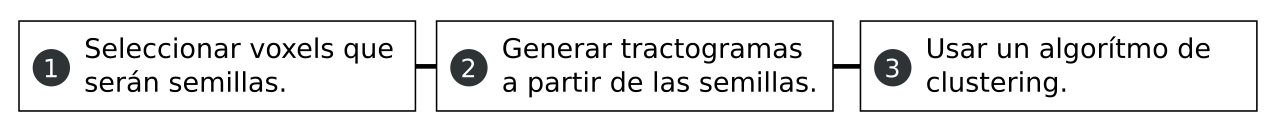
\includegraphics[width=\textwidth]{img/diagrama.png}
\caption{\textit{Pipeline} general del proceso de parcelaci\'on de la corteza cerebral.}
\label{fig:diagrama}

\end{figure}  

\section{Adquiriendo datos de los sujetos}
\label{sec:hcp}

El primer paso para parcelar la corteza cerebral de un sujeto es conseguir
tanto su imagen anat\'omica como de difusi\'on. Actualmente existen bases
de datos de gran calidad como es por ejemplo \textit{Human Connectome
Project}. \cite{VanEssen2012} Las ventajas de utilizar estos datos son
muchas: Tanto la imagen de difusi\'on como la anat\'omica se encuentran ya
preprocesadas \cite{Glasser2013}; cada sujeto posee una parcelaci\'on que,
entre otras cosas, permite separar la materia blanca de la gris; y cada
sujeto posee una superficie que representa su corteza cerebral. A su vez,
hacer uso de una base de datos p\'ublica permite reproducir con mayor
facilidad el estudio realizado.\\

\section{Seleccionando voxels que ser\'an semillas}

Como ya dijimos, la materia gris est\'a compuesta principalmente por neuronas,
y la materia blanca por axones que las comunican. Como cada neurona
posee asociado un ax\'on, colocar semillas en la interfaz entre la materia gris
y la blanca permite caracterizar las neuronas de la corteza \cite{Mori2002}
\cite{Anwander2006}. Cibu et al. \cite{Thomas2014} muestran que la materia blanca
cercana a la materia gris est\'a interconectada por peque\~nos axones. Como
estamos interesados en realizar un estudio de las conexiones entre regiones
distantes del cerebro, decidimos situar las semillas a \textit{3mm} de la corteza,
evitando as\'i el efecto de \'estos axones locales. El problema es que la corteza
del cerebro no es uniforme, sino que est\'a llena de surcos y circunvoluciones. 
Calcular la distancia entonces no es inmediato, necesita un m\'etodo que tome
estas propiedades en cuenta. A continuaci\'on presentamos el m\'etodo
\textit{Fast Marching Method} y como es posible utilizarlo para posicionar las
semillas respetando la forma de la materia blanca. \\

\textit{Fast Marching Method} es un m\'etodo para resolver num\'ericamente una
versi\'on restringida de la ecuaci\'on \textit{Eikonal}. La misma, en su forma
general, es una ecuaci\'on diferencial no lineal que se encuentra com\'unmente 
en problemas de propagaci\'on de onda. Tiene la forma: 

$$ V(x) | \nabla u(x) | = F(x) , x \in \Omega $$ 

Donde $\Omega$ es un subconjunto abierto de $R^n$ con un
\textit{buen comportamiento} en su borde. $F(x)$ se denomina el costo temporal y
$V(x)$ es la velocidad de la onda en cada punto. En el caso particular que
queremos resolver $u(x_\omega) = 0, x \in \delta\Omega$;  $F(x)=1$ y $V(x)=1$,
por lo que la ecuaci\'on se resume a:

$$ | \nabla u(x) | = 1 , x \in \Omega $$ 

$u(v)$ en este caso representa el tiempo que tarda la onda en llegar desde
alg\'un elemento del borde hasta el punto $v$ movi\'endose a velocidad constante
de una unidad de espacio por unidad de tiempo. Dada la forma de la velocidad, 
$u(v)$ tambi\'en representa \textbf{la distancia mas corta que existe entre cualquier
punto $v$ de la imagen y el borde de $\Omega$}. Dependiendo la orientaci\'on que 
se elija, las distancias a los puntos internos de la superficie ser\'an negativas
y las distancias a los puntos externos positivas (Figura \ref{fig:fmm}). 
\textit{FMM} resuelve este problema en tiempo $O(n log(n))$ \cite{Sethian2001},
siendo $n$ la cantidad de voxels de la imagen.\\

\begin{figure}[h!]

\centering
\begin{minipage}[b]{0.7\textwidth}
    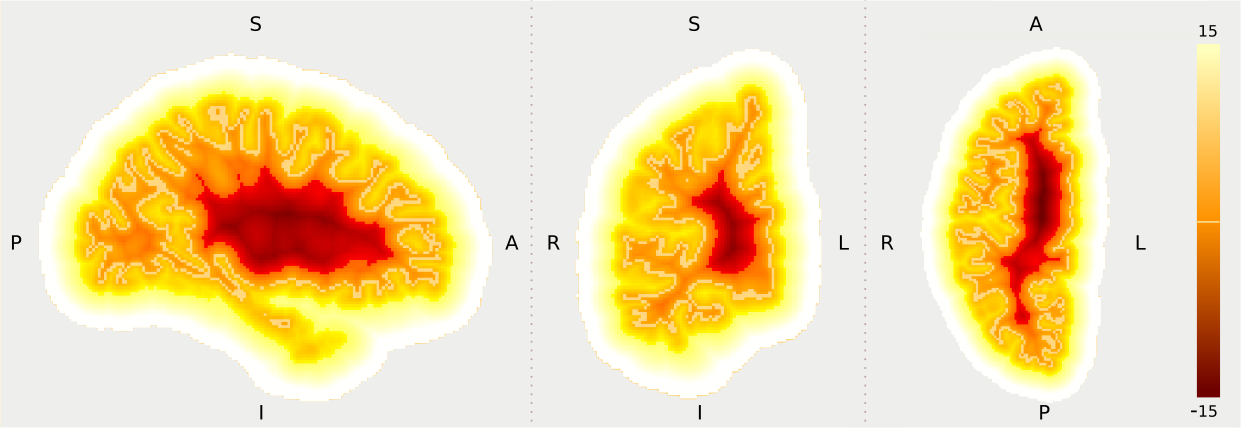
\includegraphics[width=\textwidth]{img/fmm.png}
    \caption{\small FMM sobre el hemisferio derecho, el borde la materia blanca fue
    resaltado intensionalmente}
    \label{fig:fmm}
\end{minipage} ~

\end{figure}  

Es posible utilizar este algoritmo para seleccionar voxels a cierta profundidad
en la materia blanca. Usando como borde la corteza cerebral podemos crear un mapa
de distancias en la materia blanca. El gradiente de este mapa de distancias es un
campo vectorial donde cada vector apunta hacia el interior de la materia blanca.
Caminar partiendo desde los puntos en la siguiendo este campo permite adentrarse 
respetando la morfolog\'ia de la materia blanca. Una ventaja de este m\'etodo es
que permite guardar un mapeo entre cada coordenada de la superficie y la semilla
que la representa. Otra ventaja es que es posible realizar todo el proceso en tiempo
$O(n log(n))$. \\


\section{Estabilidad algor\'itmica}
\label{sec:estabilidad}

Un tractograma es una imagen donde cada voxel representa la probabilidad de que
ese punto del cerebro est\'e conectado a la semilla elegida mediante un conjunto
de axones. Una forma de crear el tractograma de una semilla es generar un gran
n\'umero de streamlines desde ella y luego calcular la frecuencia de visitas por
cada voxel. Se denomina \textit{streamline} al camino que puede realizar una
part\'icula de agua siguiendo un mapa probabil\'istico de transiciones entre voxels.
Es importante destacar que el estimar los tractogramas de esta manera genera un 
sesgo respecto a la distancia. Cuanto m\'as lejos est\'a un voxel mayor es el 
n\'umero de transiciones probabil\'isticas necesarias para llegar a \'el. \\

Dipy es una librer\'ia para python que contiene, entre otras herramientas,
varios algoritmos para generar \textit{streamlines}. Para este trabajo elegimos
utilizar la implementaci\'on de \textit{LocalTracking} (LT de aqu\'i en mas) que
se encuentra en el paquete \textit{dipy.tracking.local}; y una implementaci\'on 
propia (MSL de aqu\'i en m\'as). Ambos algoritmos poseen una estructura 
similar: Encuadran la imagen de difusi\'on en un modelo; crean un objeto que les
permita seleccionar una direcci\'on hacia donde caminar en base a la posici\'on
actual y se mueven hasta cumplir un criterio de parada.\\

En ambos casos modelamos la informaci\'on de dMRI usando el \textit{Constrained
Spherical Deconvolve Model}. La principal diferencia entre los algoritmos surge
en la forma en que seleccionan c\'omo avanzar. Dado el conjunto de direcciones 
iniciales, esto es, las direcciones posibles a tomar desde la semilla,
LT intenta en sucesivas repeticiones del experimento elegir una distinta, 
usando as\'i todas al menos una vez. MSL por otro lado selecciona una al
azar cada vez que repite el experimento. A su vez, LT utiliza un criterio de 
parada basado en la anisotrop\'ia de la difusi\'on; MSL usa una mascara ya 
predefinida. Para mayores detalles referirse al Anexo\\

Algunas preguntas interesantes a realizar sobre los tractogramas son: ¿Al repetir
el experimento, podremos obtener el mismo tractograma?; ¿Cu\'antas part\'iculas son
necesarias para ello? y ¿Qu\'e tanto difieren los resultados entre los distintos 
algoritmos de tractograf\'ia?\\

Para determinar si los algoritmos se estabilizaban y el n\'umero de part\'iculas
necesario para que eso suceda utilizamos la t\'ecnica estad\'istica de
\textit{bootstrap} \cite{Efron1982}. Bootstrap es una forma de aproximar la
distribuci\'on del muestreo de un estad\'istico en base a calcular el mismo
utilizando sucesivos remuestreos de los datos con repeticiones. Esto es
especialmente \'util cuando el n\'umero de muestras que se posee de la poblaci\'on
no es significativamente alto. En nuestro caso situamos mas de setecientas
semillas en el \'Area de Broca y luego generamos quince mil streamlines por cada
una. Luego calculamos el tractograma medio y la varianza de cada voxel utilizando
mil submuestras aleatorias del mismo tama\~no. Esto se repiti\'o con varios
tama\~nos de submuestra para estudiar as\'i la variabilidad a medida que la
cantidad de part\'iculas crec\'ia.\\


\section{Clustering de semillas: Moreno-Dominguez.}

Moreno-Dominguez et al. \cite{Moreno-Dominguez2014} implementan el algoritmo
\textit{Agglomerative Hierarchical Clustering} para agrupar los tractogramas. 
En este algoritmo, cada \textit{feature} comienza en un cluster distinto. Luego,
el algoritmo selecciona iterativamente dos clusters siguiendo alg\'un criterio
de similitud; los agrupa en un nuevo cluster y crea un elemento representativo
de este. La jerarqu\'ia resultante de agrupar todos los clusters es expresada
como un dendrograma. En el trabajo de Moreno-Dominguez utilizan como medida de
similitud la distancia coseno (Ecuaci\'on \ref{eq:cosine}) y como criterio de
\textit{linkage} el centroide (Ecuaci\'on \ref{eq:centroide}).

\begin{figure}[h!]
                                                                                                                        
\begin{minipage}[b]{0.49\textwidth}
    \begin{equation}
        \label{eq:cosine}
        simil_{cos}(X,Y) = 1 - \frac{ X \cdot Y }{||X|| ||Y||}
    \end{equation}
\end{minipage} ~
\hfill
\begin{minipage}[b]{0.49\textwidth}
    \begin{equation}
        \label{eq:centroide}
        centroide(X,Y) = \frac{ n_X X + n_Y Y}{n_X + n_Y}
    \end{equation}
    %\caption{\small $X, Y \in R^m; n_Z = #Z$}
\end{minipage} ~

\centering
\vspace{0.5cm}
\small{$X, Y \in R^m$, $n_z = \#z$}

\end{figure}  

Para mejorar los resultados del \textit{clustering} realizan distintos tipos de
preprocesamiento en varias etapas. Aqu\'i daremos solo una breve descripci\'on 
de los mas relevantes, para mayores detalles favor de referirse al paper. \\

Una de las primeras modificaciones es al algoritmo 
\textit{Agglomerative Hierarchical Clustering}. Dado un n\'umero $k$,
las primeras $k$ iteraciones son entre clusters vecinos y de tama\~no similar.
Esto es, solo los clusters que se encuentran a menos de cierta distancia f\'isica
en el cerebro pueden ser unidos. A su vez, solo se unen los clusters que poseen
un tama\~no similar para que el dendrograma crezca de manera balanceada. \\


\settowidth\mylen{procedure Clustering(}
\addtolength\mylen{\parindent}

\begin{algorithm}[h]
\caption{Modificaciones al algoritmo Agglomerative Hierarchical Clustering.}
\label{alg:morenoahc}
\begin{algorithmic}[1]

\Procedure{Clustering(k\_pasos: primeros K pasos, \\ \hspace*{\mylen}
                      tractogramas: mat. de tractogramas, \\ \hspace*{\mylen}
                      vecinos: mat. de vecinos, \\ \hspace*{\mylen}
                      distancias: mat. de distancia clusters ) }{}
                      
    \State \emph{jerarquia} $\gets \emptyset$
                      
\For{\emph{k} in [1, cant(\emph{tractogramas})] }

    \If{\emph{k} $>$ \emph{k\_pasos}}

        \State \emph{$C_x$, $C_y$} $\gets$ clusters tales que $x$ e $y$ poseen \emph{distancia} minima      
            
    \Else{}

        \State \emph{$C_x$, $C_y$} $\gets$ $x$ e $y$ son \emph{vecinos}; 
                                   de \emph{distancia} minima y de tama\~no similar.

    \EndIf
    
    \State {tractogramas} $\gets$ eliminar clusters $C_x$, $C_y$

    \State {centroide} $\gets$ computar explicitamente el centroide $(C_x,C_y)$ 

    \State {tractogramas} $\gets$ agregar \emph{centroide}
    
    \State \emph{jerarquia} $\gets$ agregar la union $(C_x,C_y)$
    
    \For{ $C_z$ in \emph{tractogramas} }
        \State \emph{D} $\gets$ computar explicitamente distancia coseno de $C_z$ al \emph{centroide}
        \State \emph{distancias} $\gets$ actualizar distancia entre $(C_x,C_y)$ y \emph{centroide} con \emph{D}
    \EndFor            
    
\EndFor

\State \Return \emph{jerarquia} 
 
\EndProcedure 

\end{algorithmic}
\end{algorithm}

\vspace{1cm}

Una vez obtenido el dendrograma proceden a eliminar las inversiones dentro del
mismo. Una inversi\'on sucede cuando se unen dos clusters con una distancia 
interna mayor a la distancia entre ellos. Las inversiones no cambian la 
jerarqu\'ia de los clusters, sino que solo complican la interpretaci\'on visual
de los datos \cite{Murtagh1985}. Una forma de eliminarlas es colapsando las 
ramas que la componen en una sola jerarqu\'ia con mas de dos elementos. Un 
ejemplo de inversi\'on y el resultado de quitarla se muestran en las Figuras 
\ref{fig:inversion} y \ref{fig:no_inversion} respectivamente. 


\begin{figure}[h!]
                                                                                                                        
\begin{minipage}[b]{0.49\textwidth}
    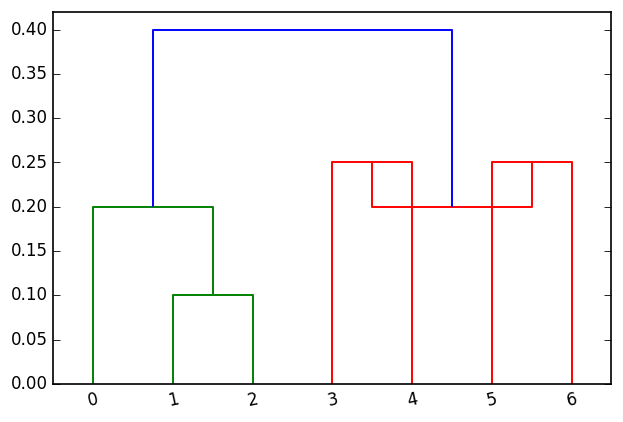
\includegraphics[width=\textwidth]{img/inversion_0.png}
    \caption{\small Dendrograma de inversi\'on.}
     \label{fig:inversion}
\end{minipage} ~
\hfill
\begin{minipage}[b]{0.49\textwidth}
    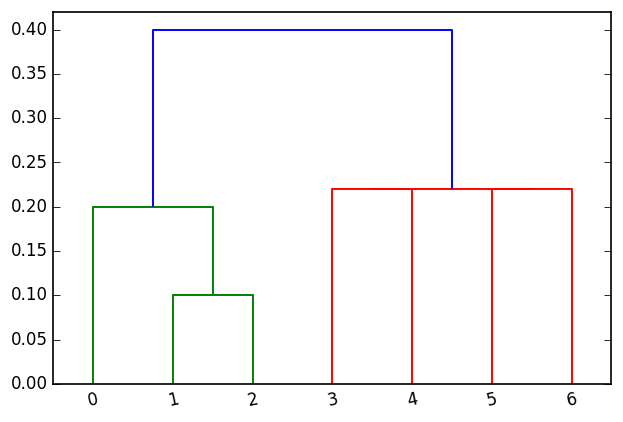
\includegraphics[width=\textwidth]{img/inversion_1.png}
    \caption{\small Dendrograma con inversi\'on corregida. }
    \label{fig:no_inversion}
\end{minipage} ~

\end{figure}  

\vspace{0.1cm}

Otro paso de preprocesamiento es el quitar \textit{outliers} del dendrograma.
Esto en realidad lo hacen durante la etapa de \textit{clustering}. Evitan que los
clusters de un solo elemento se unan a otros clusters si la (di)similitud es 
mayor a cierto \textit{threshold}. Al hacer este paso durante el \textit{clustering}
previenen que los \textit{ouliers} afecten la forma de los nuevos centroides.\\

Una vez finalizados todos los pasos el resultado es un dendrograma. Para parcelar
la corteza solo es necesario seleccionar una altura en la cual cortar dicho
dendrograma. Los clusters que est\'en por debajo de ese corte ser\'an las distintas
parcelas. \\


